\section{Experiments}
First, we compare the results of different face gradient reconstruction. Then we conduct several experiments to show that how parameters effect the  results.
\subsection{Comparison of different gradient reconstruction}
\begin{center}
    \includegraphics[width=4.8in]{images/3cmp.png}
    \fcaption{The effects of different gradient reconstruction: (a) Source face image. (b) Target face image. (c) Fusing face by linearly combining the gradients of two faces. (d) Fusing face by keeping the larger gradients of two faces. (e) Fusing face through weaker gradient preserving method.}
\end{center}

Fig. 4 shows the effects of different face gradient reconstruction. From Fig. 4(c), we can see that direct linear combination of  gradients of two faces could bring too much illumination from the source face into the target face, which makes face look very unnatural. If we kept the stronger gradients of two faces, the lightning condition of the target face would be strongly broken. More importantly, we can't control how much features we are going to fuse from the source face into the target face. In Fig. 4(e), the lightning condition and facial hues is closest to the target face image among all the results. When we reconstruct gradients using the proposed algorithm, we only keep the stronger gradients of the source face, which means the main features of the source are preserved.

\subsection{How the different parameters effect face fusion}
 For our task, there are four parameters we can adjust, they are $\alpha$, $\beta$, $\theta_1$, $\theta_2$. $\alpha$ controls the structure of human faces, in other words, it controls the profile and the distribution of features of human faces. $\beta$ controls the details of human faces, like wrinkles and textures. With $\alpha$ and $\beta$, we can control how much content we want to fuse from source face into target face. If the gradients of source face is weaker than $\theta_1$ and the gradients of target face is weaker than $\theta_2$, then we retain the gradients of the target face. Otherwise, we keep the gradients of the source face.

Fig. 5 shows how $\alpha$ effects the fused results, $\beta = 0.5$, $\theta_1 = 10$, $\theta_2 = 15$. As the $\alpha$ grows bigger, the distribution of face features of fused face is more like the source face.

\begin{center}
    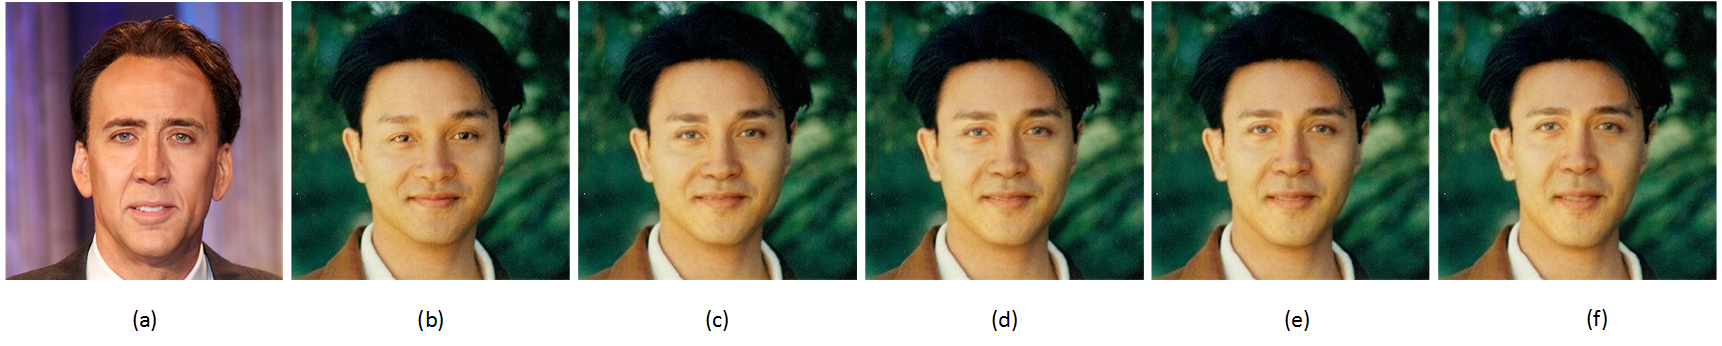
\includegraphics[width=4.8in]{images/pro.png}
    \fcaption{(a) Source face. (b) Target face. (c) Fused face, $\alpha = 0.2$. (d) Fused face, $\alpha = 0.4$. (e) Fused face, $\alpha = 0.6$. (f) Fused face, $\alpha = 0.8$.}
\end{center}

Fig. 6 shows how $\beta$ effects the fused result. $\alpha = 0.5$, $\theta_1 = 10$, $\theta_2 = 15$. As the $\beta$ grows bigger, the fused result has more details from source face.

\begin{center}
    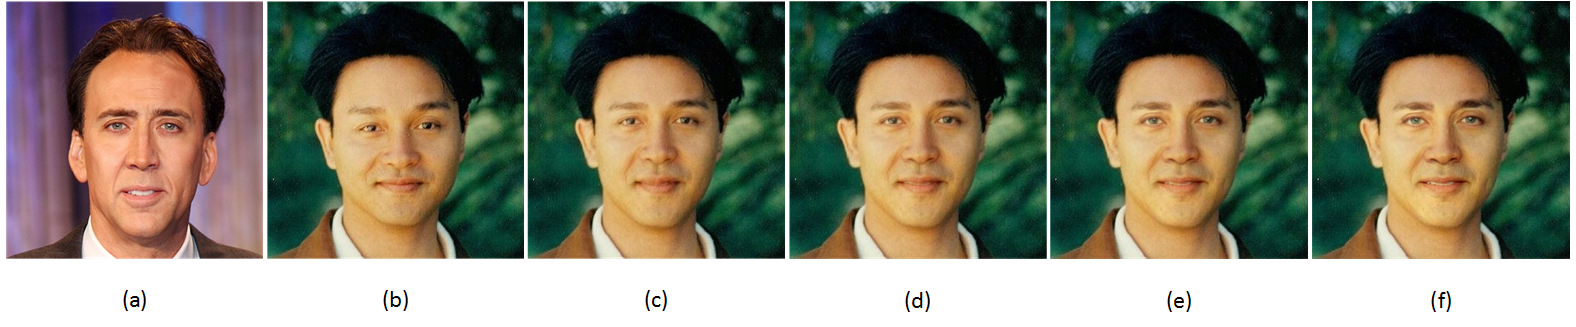
\includegraphics[width=4.8in]{images/detail.png}
    \fcaption{(a) Source face. (b) Target face. (c) Fused face, $\beta = 0.2$. (d) Fused face, $\beta = 0.4$. (e) Fused face, $\beta = 0.6$. (f) Fused face, $\beta = 0.8$.}
\end{center}

If we want to only keep main features of source face, we could only retain stronger gradients of the source face, Fig. 7 shows that the fused results are more natural as more weaker gradients of the source face are been dropped. $\alpha = 0.5$, $\beta = 0.5$, $\theta_2 = 40$. The weaker gradients carry too much illumination information and facial hues of the source face, when these gradients are brought into the fused results, the results become very unnatural.

\begin{center}
    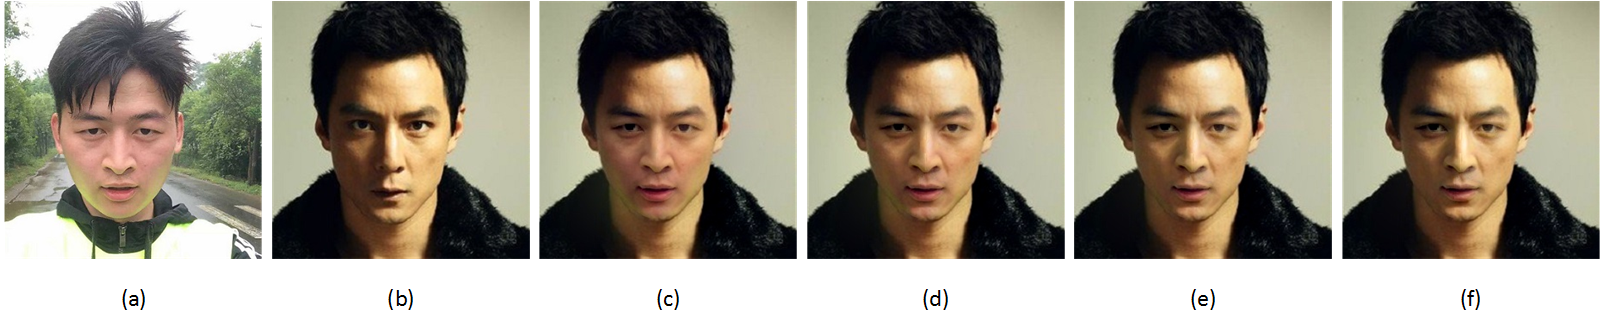
\includegraphics[width=4.8in]{images/thd1.png}
    \fcaption{(a) Source face. (b) Target face. (c) Fused face, $\theta_1 = 2$. (d) Fused face, $\theta_1 = 4$. (e) Fused face, $\theta_1 = 6$. (f) Fused face, $\theta_1 = 8$.}
\end{center}

When we fuse the main features of source face into target face, somehow, we need to erase the main features of target face. In fact, we want to keep the illumination information of the target face, both the weaker gradients of source face and weaker gradients of target face are preserved. For Fig. 8, it shows the experiment on $\theta_2$,  $\alpha = 0.5$, $\beta = 0.5$, $\theta_1 = 10$, when the $\theta_2$ grows bigger, more stronger gradients are preserved. As we can see, more shadows are preserved.

\begin{center}
    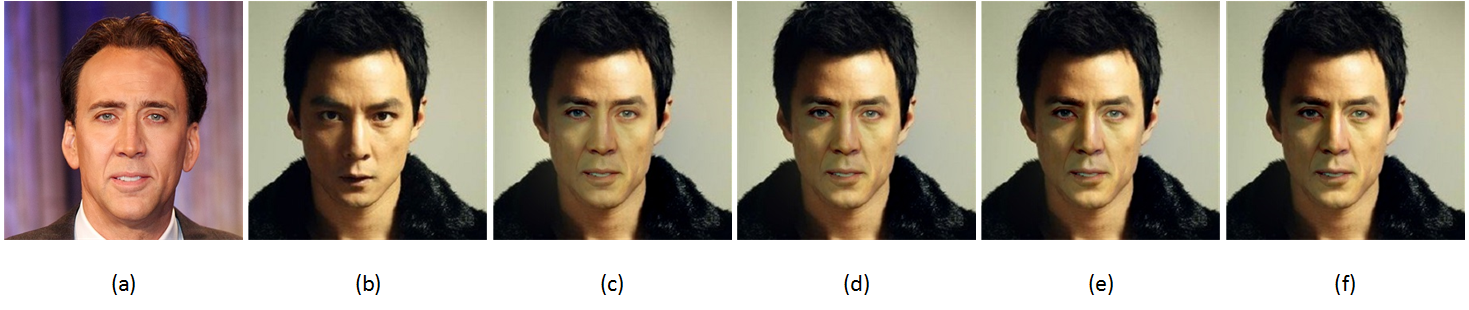
\includegraphics[width=4.8in]{images/thd2.png}
    \fcaption{(a) Source face. (b) Target face. (c) Fused face, $\theta_2 = 10$. (d) Fused face, $\theta_2 = 20$. (e) Fused face, $\theta_2 = 30$. (f) Fused face, $\theta_2 = 40$.}
\end{center}

Although our work are not aiming at face swapping task, we still could create similar effects by setting $\beta = 1$. This means we almost preserving all the gradients of source faces, but only keep part of weaker gradients of target faces. We compare our results and the work of Korshunova et al. \cite{faceswapping}. In Fig. 9, the source face of all the results is from Fig. 8(a), we can see that our results keep more illumination information and facial hues of target faces which makes our results more natural. But in Fig. 9(c), our result fail to catch the lightning condition of the target face from a high level, this is where we need improve.

\begin{center}
    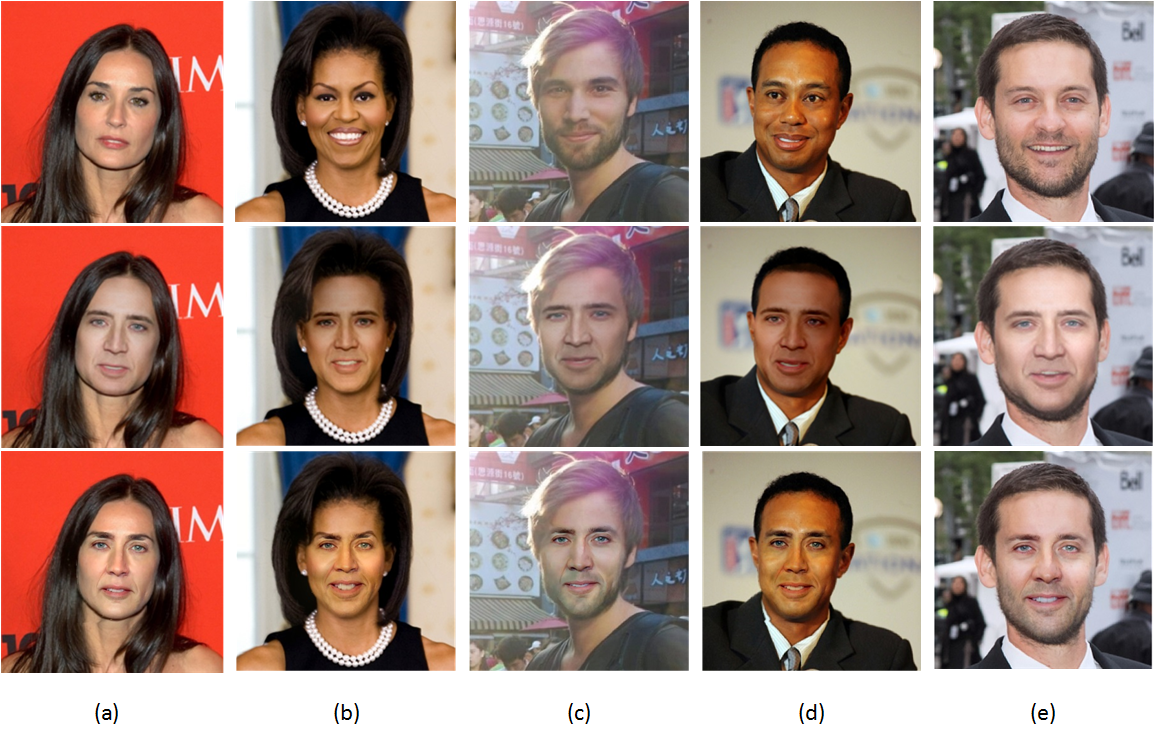
\includegraphics[width=4.8in]{images/vs.png}
    \fcaption{The first row are the original target face, the second row are the results of Korshunova et al., the third row are our results. Our algorithm preserves more illumination information and facial hues of target face.}
\end{center}

In Fig. 10, as $\alpha$ and $\beta$ grow bigger, the output faces have more features from the source face.

\begin{center}
    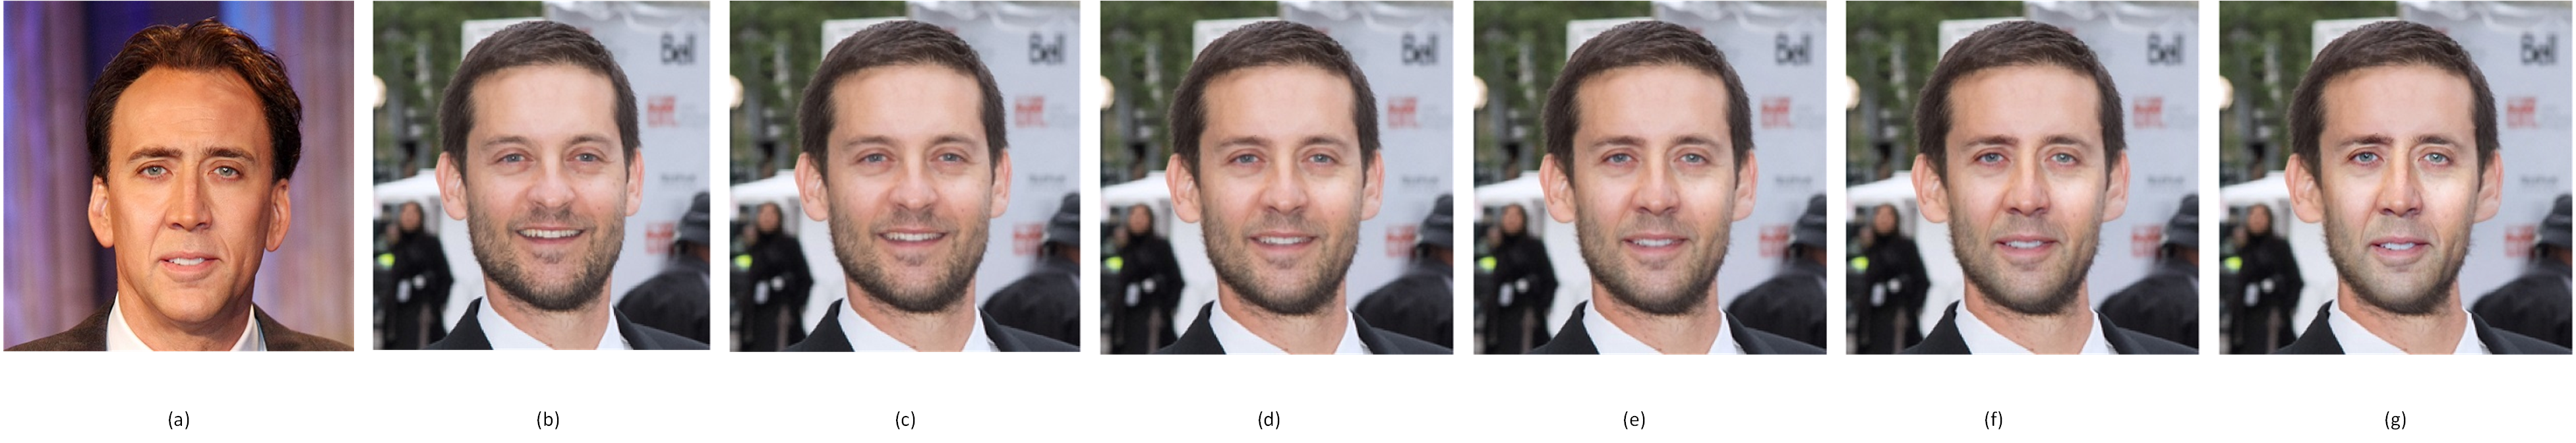
\includegraphics[width=4.8in]{images/trans.png}
    \fcaption{(a) Source face. (b) Target face. (c) Fused face, $\alpha = 0.2$, $\beta = 0.2$. (d) Fused face, $\alpha = 0.4$, $\beta = 0.4$. (e) Fused face, $\alpha = 0.6$, $\beta = 0.6$. (f) Fused face, $\alpha = 0.8$, $\beta = 0.8$. (g) Fused face, $\alpha = 1$, $\beta = 1$.}
\end{center}
